\begin{figure}
  \centering
  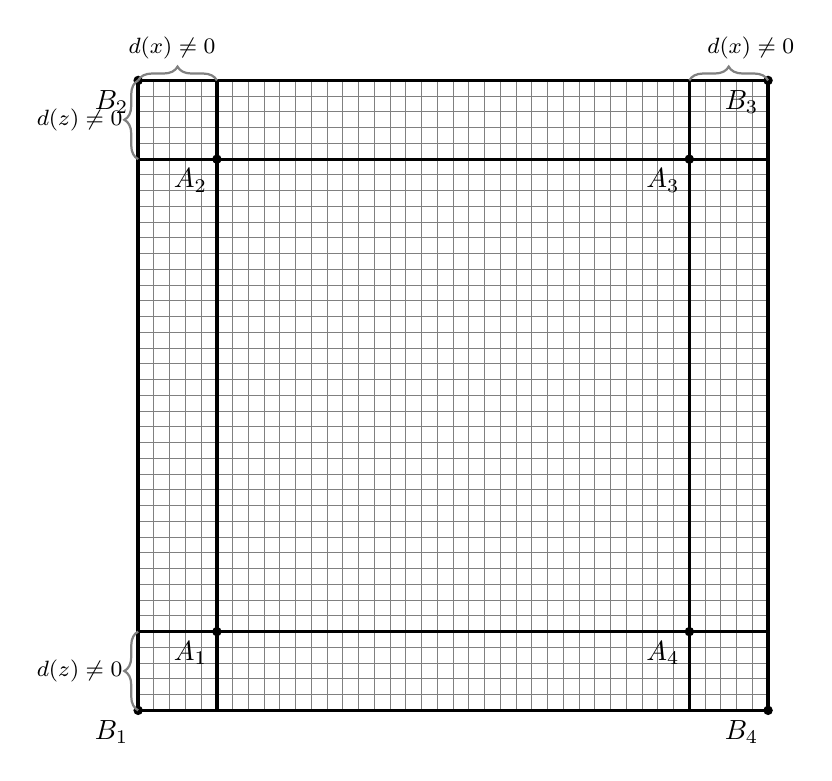
\begin{tikzpicture}
    \draw[step=0.2cm,color=gray] (-4,-4) grid (4,4);
    \draw[below left] (-3,-3) node(s){$A_1$};
    \draw[below left] (-3,3) node(s){$A_2$};
    \draw[below left] (3,3) node(s){$A_3$};
    \draw[below left] (3,-3) node(s){$A_4$};
    \draw[below left] (-4,-4) node(s){$B_1$};
    \draw[below left] (-4,4) node(s){$B_2$};
    \draw[below left] (4,4) node(s){$B_3$};
    \draw[below left] (4,-4) node(s){$B_4$};
    \draw[very thick] (-3,-4)--(-3,4);    
    \draw[very thick] (3,-4)--(3,4);
    \draw[very thick] (-4,3)--(4,3);    
    \draw[very thick] (-4,-3)--(4,-3);
    \draw[very thick] (-4,-4)--(-4,4)--(4,4)--(4,-4)--cycle;   
    \fill (-3,-3) circle (0.06cm) (-3,3) circle (0.06cm) (3,3) circle (0.06cm) (3,-3)circle (0.06cm);
    \fill (-4,-4) circle (0.06cm) (-4,4) circle (0.06cm) (4,4) circle (0.06cm) (4,-4)circle (0.06cm); 
    
    \draw [thick,gray,decorate,decoration={brace,amplitude=5pt}] (-4,4)  -- (-3,4) 
      node [black,midway,above=4pt,xshift=-2pt] {\footnotesize $d(x)\neq 0$};
    \draw [thick,gray,decorate,decoration={brace,amplitude=5pt}] (3,4) -- (4,4)
      node [black,midway,above=4pt,xshift=8pt] {\footnotesize $d(x)\neq 0$};
    \draw [thick,gray,decorate,decoration={brace,amplitude=5pt}] (-4,-4)  -- (-4,-3) 
      node [black,midway,left=10pt,xshift=8pt] {\footnotesize $d(z)\neq 0$};
    \draw [thick,gray,decorate,decoration={brace,amplitude=5pt}] (-4,3) -- (-4,4)
      node [black,midway,left=10pt,xshift=8pt] {\footnotesize $d(z)\neq 0$};
  \end{tikzpicture}
  \caption{A schematic diagram of extended artificial boundary area. $A_1A_2A_3A_4$ is the original model zone, which is extended to be $B_1B_2B_3B_4$  with artificial boundary. In the extended bounary area, the attenuation coeffcient $d(u)\neq 0$; In the model zone $A_1A_2A_3A_4$, $d(u)= 0$, $u=x,z$. }\label{fig:extbndr}
\end{figure}

